Trois idées ont été étudiées pour le déplacement des \glspl{microcapsule} de la \gls{wellplate} jusqu'au réacteur. 
Pour le déplacement des \glspl{microcapsule} de leur plaque jusqu'aux réacteurs, trois idées ont été étudiées : 
\begin{itemize}
    \item Transport pneumatique par tube;
    \item convoyeur;
    \item robot.
\end{itemize}
\subsection*{Transport pneumatique par tube}
Le système de transport pneumatique par tube serait des tuyaux dans lesquels naviguent les \glspl{microcapsule} grâce à une différence de pression de chaque côté de la \gls{microcapsule}. Ce système est déjà présent dans les hôpitaux et dans les grandes surfaces.
\begin{figure}[ht]
    \centering
    \begin{subfigure}{0.45\textwidth}
        \centering
        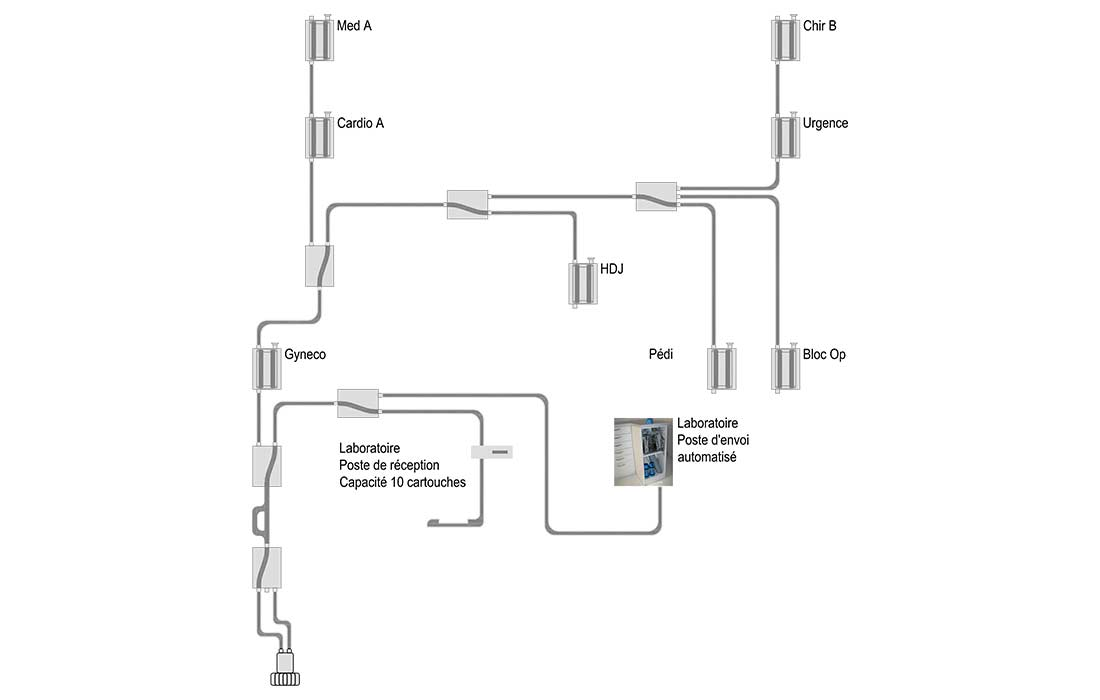
\includegraphics[width=\linewidth]{assets/figures/Hardware/transport_pneu/reseau_pneumatique_hopital.jpg}
        \caption{Schéma d'un réseau de transport pneumatique\footnotemark}
    \end{subfigure}\hfill
    \begin{subfigure}{0.45\textwidth}
        \centering
        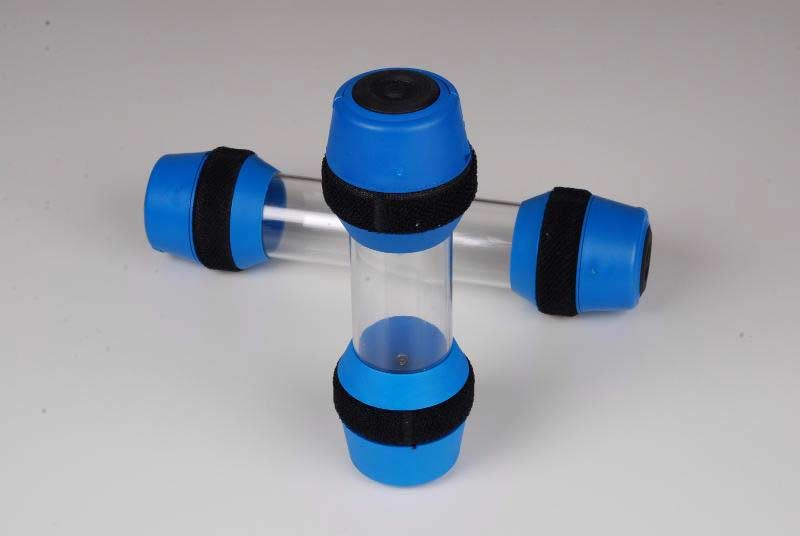
\includegraphics[width=\linewidth]{assets/figures/Hardware/transport_pneu/cartouche_transport_pneu.jpg}
        \caption{Cartouche de transport\footnotemark}
    \end{subfigure}
    \caption{Exemples de réseau de transport pneumatique par tube}
\end{figure}
\footnotetext[3]{\href{https://www.transport-pneumatique.fr/transport-pneumatique-centres-hospitaliers/}{https://www.transport-pneumatique.fr/transport-pneumatique-centres-hospitaliers/}}
\footnotetext[4]{\href{https://www.transport-pneumatique.fr/cartouches-pochettes/}{https://www.transport-pneumatique.fr/cartouches-pochettes/}}
\subsection*{Transport par convoyeur}
Pour déplacer les \glspl{microcapsule}, un convoyeur peut être utilisé, il faut néanmoins que le convoyeur soit adapté au \gls{microcapsule}, les \glspl{microcapsule} étant cylindriques, elles risqueraient de rouler sur un convoyeur à bande lisse, mais une bande à tasseau (\cf \autoref{img:convoyeur_bande_tasseau}) ou un demi-tube  (\cf \autoref{img:convoyeur_tube}) conviendraient parfaitement.
\begin{figure}[ht]
    \centering
    \begin{subfigure}{0.45\textwidth}
        \centering
        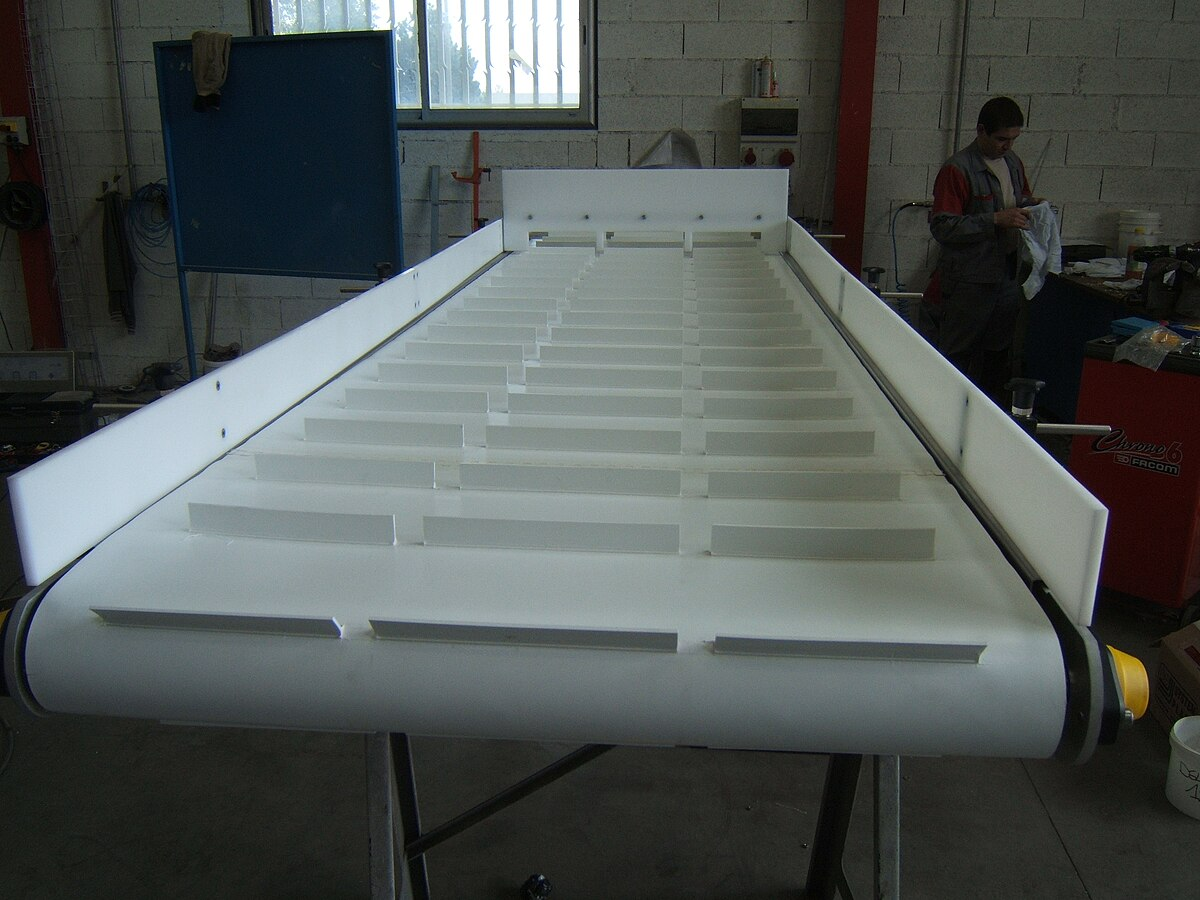
\includegraphics[width=\linewidth]{assets/figures/Hardware/transport_conv/convoyeur_tasseau.JPG}
        \caption{Convoyeur avec bande à tasseaux\footnotemark}
        \label{img:convoyeur_bande_tasseau}
    \end{subfigure}\hfill
    \begin{subfigure}{0.45\textwidth}
        \centering
        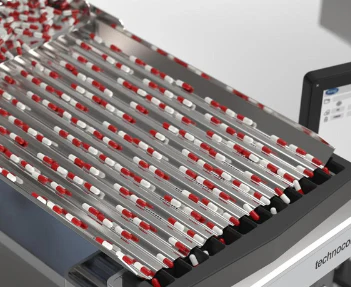
\includegraphics[width=\linewidth]{assets/figures/Hardware/transport_conv/convoyeur_tube.png}
        \caption{Convoyeur à tube\footnotemark}
        \label{img:convoyeur_tube}
    \end{subfigure}
    \caption{Exemple de convoyeur}
\end{figure}
\footnotetext[5]{\href{https://fr.m.wikipedia.org/wiki/Convoyeur}{https://fr.m.wikipedia.org/wiki/Convoyeur}}
\footnotetext[6]{\href{https://doser-compter.com/products/ligne-de-comptage-king}{https://doser-compter.com/products/ligne-de-comptage-king}}
Quant aux différents moyens de mouvoir les \glspl{microcapsule}, il y a : 
\begin{itemize}
    \item les vibrations;
    \item le déplacement de la bande;
    \item la gravité.
\end{itemize}

La dernière option nécessite des surfaces lisses, que le système soit en pente et le temps de déplacement n'est pas réglable. Les deux autres solutions ne se distinguent pas vraiment pour l'instant, car dans tous les cas, l'utilisation d'un moteur électrique est nécessaire.

\subsection*{Déplacement à l'aide d'un robot}
Pour le déplacement des \glspl{microcapsule}, seuls les axes $T_x, T_y~\text{et}~T_z$ sont nécessaires, soit $3$ degrés de liberté. Un robot de type \textit{SCARA}, cylindrique ou Delta peuve correspondre.

\subsection*{Avantages et inconvénients}
\begin{table}[H]
    \caption{Anvantages et inconvénients des solutions de transport des \glspl{microcapsule}}
    \begin{tabular}{@{}cll@{}}
    \toprule
    Solution      & \multicolumn{1}{c}{Avatanges}                                                                                                   & \multicolumn{1}{c}{Inconvénient}                                                                                                                                  \\ \midrule
    Transport pneumatique par tube    & \begin{tabular}[c]{@{}l@{}} - Peu de mouvements mécaniques\end{tabular} & \begin{tabular}[c]{@{}l@{}}- Peu modulable\\ - Bruyant\\ - Aiguillage complexe\end{tabular}                                                                     \\
    Convoyeur & \begin{tabular}[c]{@{}l@{}}\end{tabular} & \begin{tabular}[c]{@{}l@{}}- Maintenance fréquente\end{tabular} \\
    Robot   & \begin{tabular}[c]{@{}l@{}}- Place\\ - Modulable \\ \end{tabular}                            & \begin{tabular}[c]{@{}l@{}}- Coût\end{tabular}     \\ \bottomrule
    \end{tabular}
\end{table}